\documentclass[journal,13pt,twocolumn]{IEEEtran}

\usepackage{setspace}
\usepackage{gensymb}
\counterwithin{equation}{section}
\singlespacing

\newcommand{\myvec}[1]{\ensuremath{\begin{pmatrix}#1\end{pmatrix}}}
\newcommand{\mydet}[1]{\ensuremath{\begin{vmatrix}#1\end{vmatrix}}}

\usepackage[cmex10]{amsmath}
\usepackage{amsthm}
\usepackage{mathrsfs}
\usepackage{txfonts}
\usepackage{stfloats}
\usepackage{bm}
\usepackage{cite}
\usepackage{cases}
\usepackage{subfig}
\usepackage{longtable}
\usepackage{multirow}
\usepackage{mathtools}
\usepackage{steinmetz}
\usepackage{tikz}
\usepackage{circuitikz}
\usepackage{verbatim}
\usepackage{tfrupee}
\usepackage[breaklinks=true]{hyperref}
\usepackage{tkz-euclide} % loads  TikZ and tkz-base
%\usetkzobj{all}
\usetikzlibrary{calc,math}
\usepackage{listings}
    \usepackage{color}                                            %%
    \usepackage{array}                                            %%
    \usepackage{longtable}                                        %%
    \usepackage{calc}                                             %%
    \usepackage{multirow}                                         %%
    \usepackage{hhline}                                           %%
    \usepackage{ifthen}                                           %%
  %optionally (for landscape tables embedded in another document): %%
    \usepackage{lscape}     
\usepackage{multicol}
\usepackage{chngcntr}
\usepackage{pgfplots}
\usepackage{pgfplotstable}
\pgfplotsset{compat=1.7}
\usepackage{tikz}
\DeclareMathOperator*{\Res}{Res}
\renewcommand\thesection{\arabic{section}}
\renewcommand\thesubsection{\thesection.\arabic{subsection}}
\renewcommand\thesubsubsection{\thesubsection.\arabic{subsubsection}}

\renewcommand\thesectiondis{\arabic{section}}
\renewcommand\thesubsectiondis{\thesectiondis.\arabic{subsection}}
\renewcommand\thesubsubsectiondis{\thesubsectiondis.\arabic{subsubsection}}

\DeclarePairedDelimiter\abs{\lvert}{\rvert} % \abs{} for numerisk værdi
\DeclarePairedDelimiter\norm{\lVert}{\rVert}
\makeatletter
\let\oldabs\abs
\def\abs{\@ifstar{\oldabs}{\oldabs*}}
\let\oldnorm\norm
\def\norm{\@ifstar{\oldnorm}{\oldnorm*}}
\makeatother
\renewcommand{\vec}[1]{\mathbf{#1}}
\newcommand{\bignorm}[1]{\Bigl \| #1 \Bigr \| #1}
\hyphenation{op-tical net-works semi-conduc-tor}
\def\inputGnumericTable{}                                 %%

\lstset{
frame=single, 
breaklines=true,
columns=fullflexible
}
\begin{document}
\title{Assignment 4} 
\author{Shweta Verma} 
\maketitle
\newpage
\bigskip
\begin{abstract}
This document determines the value of $k$ for which the given equation represents a pair of straight lines.
\end{abstract}
\section{\textbf{Problem}}
For what value of $k$ does the equation 
\begin{align}
\vec{x}^T \myvec{6 && k/2 \\ k/2 && -3} \vec{x} + \myvec{4 && 5}\vec{x} -2 = 0
\end{align}
represent a pair of straight lines?
\section{\textbf{Solution}}
Equation (1.1) can also be written as 
\begin{align}
\vec{x}^T \myvec{a && b \\ b && c} \vec{x} + \myvec{d && e}\vec{x} + f = 0
\end{align}
\begin{equation}
\vec{V}=\myvec{6 && k/2\\ k/2 && -3}
\end{equation}
\begin{equation}
\vec{u}=\myvec{2\\5/2}\\
\end{equation}
\begin{equation}
f= -2
\end{equation}
Block Matrix
\begin{align}
 = \myvec{6 && k/2 && 2\\ k/2 && -3 && 5/2\\2 && 5/2 && -2}
\end{align}
Determinant of the Block Matrix
\begin{align}
\Delta = \mydet{6 && k/2 && 2\\ k/2 && -3 && 5/2\\2 && 5/2 && -2}
\end{align}
If the equation (1.1) represents a pair of straight lines\\
then the Determinant is zero
\begin{align}
\Delta = 0
\end{align}
\begin{align}
\implies \mydet{6 && k/2 && 2\\ k/2 && -3 && 5/2\\2 && 5/2 && -2} = 0
\end{align}
\begin{align}
\implies 6\times(6-25/4)-k/2(-k-5)+2(5k/4+6) = 0
\end{align}
\begin{align}
\implies k^2 + 10k + 21 = 0
\end{align}
\begin{align}
\implies \boxed{ k = -3 }
\end{align}
\begin{align}
\implies \boxed{ k = -7 }
\end{align}
Substituting k=-3 in (1.1)
\begin{align}
\vec{x}^T \myvec{6 && -3/2 \\ -3/2 && -3} \vec{x} + \myvec{4 && 5}\vec{x} -2 = 0
\end{align}
Equation (2.12) can be represented as 
\begin{align}
\vec{V}=\myvec{6 && -3/2\\ -3/2 && -3}
\end{align}
\begin{align}
\vec{u}=\myvec{2\\5/2}
\end{align}
\begin{align}
f= -2
\end{align}
The pair of Straight lines can be given by
\begin{align}
(\vec{n_1}^T\vec{x}-c_1)(\vec{n_2}^T\vec{x}-c_2)=0
\end{align}
Using (2.12) and (2.16)
\begin{align}
(\vec{n_1}^T\vec{x}-c_1)(\vec{n_2}^T\vec{x}-c_2)= \vec{x}^T \myvec{6 && -3/2 \\ -3/2 && -3} \vec{x} + \myvec{4 && 5}\vec{x} -2
\end{align}
Comparing both sides,
\begin{align}
\vec{n_1}c_2 + \vec{n_2}c_1 = -\myvec{4 \\ 5}\\
c_1c_2 = -2
\end{align}
The slope of the lines can be given by the roots of the polynomial:
\begin{align}
cm^2 + bm + a = 0\\
\implies m_i=\frac{-b\pm\sqrt{-det(V)}}{c}
\end{align}
\begin{align}
\vec{n_i} = k_i\myvec{-m_i \\ 1}
\end{align}
Substituting values in (2.21) and (2.22)
\begin{align}
-3m^2 -3m +6 = 0\\
\implies m_i = \frac{\frac{-3}{2}\pm \frac{9}{2}}{3}\\
\implies m_1 = 1 , m_2 = -2
\end{align}
Therefore,
\begin{align}
\vec{n_1} = k_1 \myvec{-1 \\ 1}\\
\vec{n_2} = k_2 \myvec{2 \\ 1}
\end{align}
we know that
\begin{align}
\vec{n_1} * \vec{n_2} =\myvec{a\\2b\\c}\\
k_1 \myvec{-1 \\ 1} *  k_2 \myvec{2 \\ 1} = \myvec{6\\-3\\-3}\\
\implies k_1k_2 = -3
\end{align}
Taking $k_1 = -3$ and $k_2 = 1$ we get
\begin{align}
\vec{n_1} = \myvec{3 \\ -3}\\
\vec{n_2} = \myvec{2 \\ 1}
\end{align}
Now to find $ c_1 $and$ c_2 $using (2.19) 
\begin{align}
\myvec{\vec{n_1} && \vec{n_2}} \myvec{c_2 \\ c_1} = -\myvec{4 \\ 5}\\
\myvec{3 && 2\\ -3 && 1}\myvec{c_2 \\ c_1} = -\myvec{4 \\ 5}
\end{align}
Row reducing the augmented matrix
\begin{align}
\myvec{3 && 2 && -4\\ -3 && 1 && -5} \xleftrightarrow[]{R_2\rightarrow R_1+R_2}\myvec{3 && 2 && -4\\ 0 && 3 && -9}\\
\xleftrightarrow[]{R_2\rightarrow R_2/3}\myvec{3 && 2 && -4\\ 0 && 1 && -2}\\
\implies \myvec{3 && 2\\ 0 && 1}\myvec{c_2 \\ c_2} = \myvec{-4 \\ -2}\\
\implies c_1 = -3 , c_2 = 2/3
\end{align}
Substituting (2.32),(2.33) and (2.39) in (2.17)\\
The equation of the lines:
\begin{align}
\boxed{(3x - 3y + 3)(2x + y - 2/3) = 0}
\end{align}
\begin{figure}
   \centering
   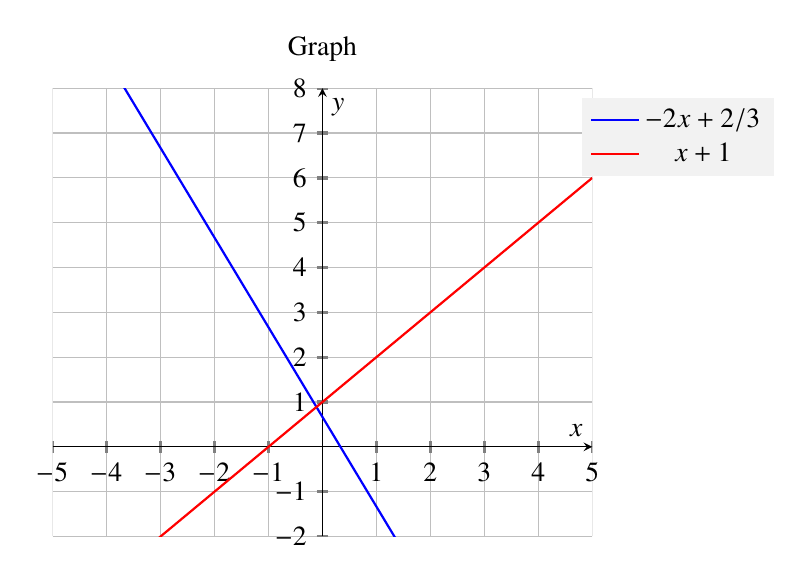
\begin{tikzpicture}
   \begin{axis}[
   legend style={anchor=north west,draw=none,fill=gray!10},
   axis lines=middle,
   grid=major,
   xmin=-5,
   xmax=5,
   ymin=-2,
   ymax=8,
   title=Graph,
   xlabel={$x$},
   ylabel={$y$},
   xtick={-5,-4,...,5},
   ytick={-2,-1,...,8},
   tick style={very thick}
   ]
   \addplot[blue,thick]{-2*x+2/3};
   \addlegendentry{$-2x+2/3$}
   \addplot[red,thick]{x+1};
   \addlegendentry{$x+1$}
   \end{axis}
   \end{tikzpicture}
   \caption{This is a plot of pair of straight lines when k=-3}
   \end{figure}
   Similarly, substituting k = -7 in (1.1)
   \begin{align}
   \vec{x}^T \myvec{6 && -7/2 \\ -7/2 && -3} \vec{x} + \myvec{4 && 5}\vec{x} -2 = 0
   \end{align}
   Equation (2.41) can be represented as 
\begin{align}
\vec{V}=\myvec{6 && -7/2\\ -7/2 && -3}
\end{align}
\begin{align}
\vec{u}=\myvec{2\\5/2}
\end{align}
\begin{align}
f= -2
\end{align}
The pair of Straight lines can be given by
\begin{align}
(\vec{n_1}^T\vec{x}-c_1)(\vec{n_2}^T\vec{x}-c_2)=0
\end{align}
Using (2.12) and (2.16)
\begin{align}
(\vec{n_1}^T\vec{x}-c_1)(\vec{n_2}^T\vec{x}-c_2)= \vec{x}^T \myvec{6 && -7/2 \\ -7/2 && -3} \vec{x} + \myvec{4 && 5}\vec{x} -2
\end{align}
Comparing both sides,
\begin{align}
\vec{n_1}c_2 + \vec{n_2}c_1 = -\myvec{4 \\ 5}\\
c_1c_2 = -2
\end{align}
The slope of the lines can be given by the roots of the polynomial:
\begin{align}
cm^2 + bm + a = 0\\
\implies m_i=\frac{-b\pm\sqrt{-det(V)}}{c}
\end{align}
\begin{align}
\vec{n_i} = k_i\myvec{-m_i \\ 1}
\end{align}
Substituting values in (2.49)
\begin{align}
-3m^2 -7m +6 = 0\\
\implies m_i = \frac{\frac{-7}{2}\pm \frac{11}{2}}{3}\\
\implies m_1 = 2/3 , m_2 = -3
\end{align}
Therefore,
\begin{align}
\vec{n_1} = k_1 \myvec{-2/3 \\ 1}\\
\vec{n_2} = k_2 \myvec{3 \\ 1}
\end{align}
we know that
\begin{align}
\vec{n_1} * \vec{n_2} =\myvec{a\\2b\\c}\\
k_1 \myvec{-2/3 \\ 1} *  k_2 \myvec{3 \\ 1} = \myvec{6\\-7\\-3}\\
\implies k_1k_2 = -3
\end{align}
Taking $k_1 = -3$ and $k_2 = 1$ we get
\begin{align}
\vec{n_1} = \myvec{2 \\ -3}\\
\vec{n_2} = \myvec{3 \\ 1}
\end{align}
Now to find $ c_1 $ and $ c_2 $using (2.19) 
\begin{align}
\myvec{\vec{n_1} && \vec{n_2}} \myvec{c_2 \\ c_1} = -\myvec{4 \\ 5}\\
\myvec{2 && 3\\ -3 && 1}\myvec{c_2 \\ c_1} = -\myvec{4 \\ 5}
\end{align}
Row reducing the augmented matrix
\begin{align}
\myvec{2 && 3 && -4\\ -3 && 1 && -5} \xleftrightarrow[]{R_2\rightarrow 3R_1+2R_2}\myvec{2 && 3 && -4\\ 0 && 11 && -22}\\
\xleftrightarrow[]{R_2\rightarrow R_2/11}\myvec{2 && 3 && -4\\ 0 && 1 && -2}
\end{align}
\begin{align}
\implies \myvec{2 && 3\\ 0 && 1}\myvec{c_2 \\ c_2} = \myvec{-4 \\ -2}\\
\implies c_1 = -2 , c_2 = 1
\end{align}
Substituting (2.32),(2.33) and (2.39) in (2.17)\\
The equation of the lines:
\begin{align}
\boxed{(2x - 3y + 2)(3x + y - 1) = 0}
\end{align}
\begin{figure}
   \centering
   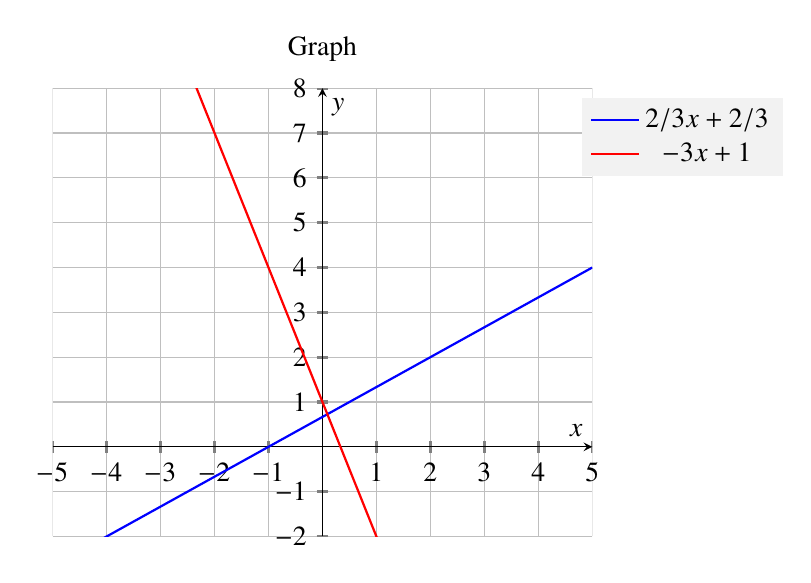
\begin{tikzpicture}
   \begin{axis}[
   legend style={anchor=north west,draw=none,fill=gray!10},
   axis lines=middle,
   grid=major,
   xmin=-5,
   xmax=5,
   ymin=-2,
   ymax=8,
   title=Graph,
   xlabel={$x$},
   ylabel={$y$},
   xtick={-5,-4,...,5},
   ytick={-2,-1,...,8},
   tick style={very thick}
   ]
   \addplot[blue,thick]{2/3*x+2/3};
   \addlegendentry{$2/3x+2/3$}
   \addplot[red,thick]{-3*x+1};
   \addlegendentry{$-3x+1$}
   \end{axis}
   \end{tikzpicture}
   \caption{This is a plot of pair of straight lines when k=-7}
   \end{figure}
\end{document} 
